\chapter{Реализация и тестирование системы}

\section{Реализация компонентов системы в виде микросервисов}

\subsection{Сущности предметной области}
В каждом микросервисе существует своя предметная область. Все ключевые сущности заданы в виде структур, для оперирования
ими в логике микросервиса.

\begin{figure}[H]%
	\begin{center}
		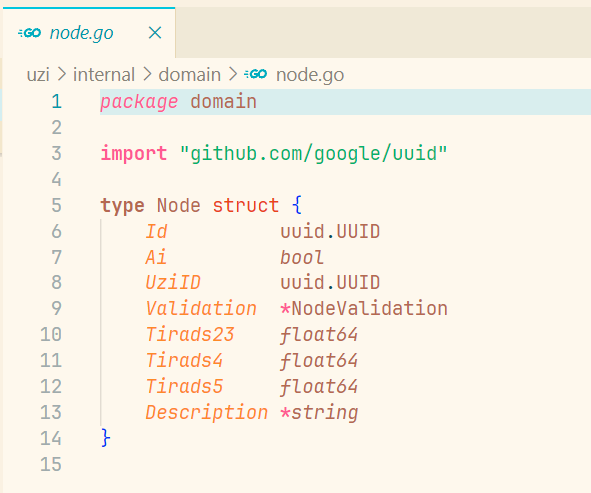
\includegraphics[width=.7\columnwidth]{./img/new/domain_node.png}%
	\end{center}
	\caption{Сущности узла образования в щитовидной железе}%
	\label{pic:domain_node}%
\end{figure}

\begin{figure}[H]%
	\begin{center}
		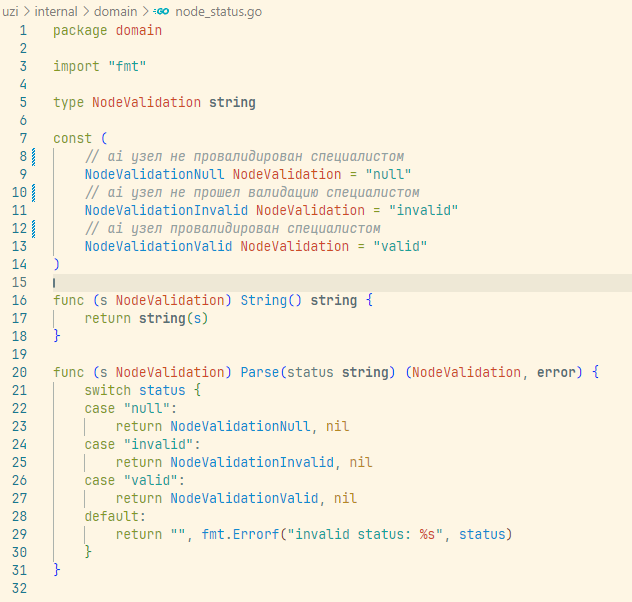
\includegraphics[width=.7\columnwidth]{./img/new/domain_node_status.png}%
	\end{center}
	\caption{Статусы узла образования в щитовидной железе}%
	\label{pic:domain_node_status}%
\end{figure}

Сущности предметной области не имеют зависимостей от внешних частей или структур системы.

\subsection{Логические сценарии использования}
Вся логика которая имеется в микросервисе реализована в этом слое приложения. Никакая логика не допустима в другом месте. 
Такой подход к разработке позволяет легко отлаживать и контролировать систему, она не <<растякается>> по всему коду.

\begin{figure}[H]%
	\begin{center}
		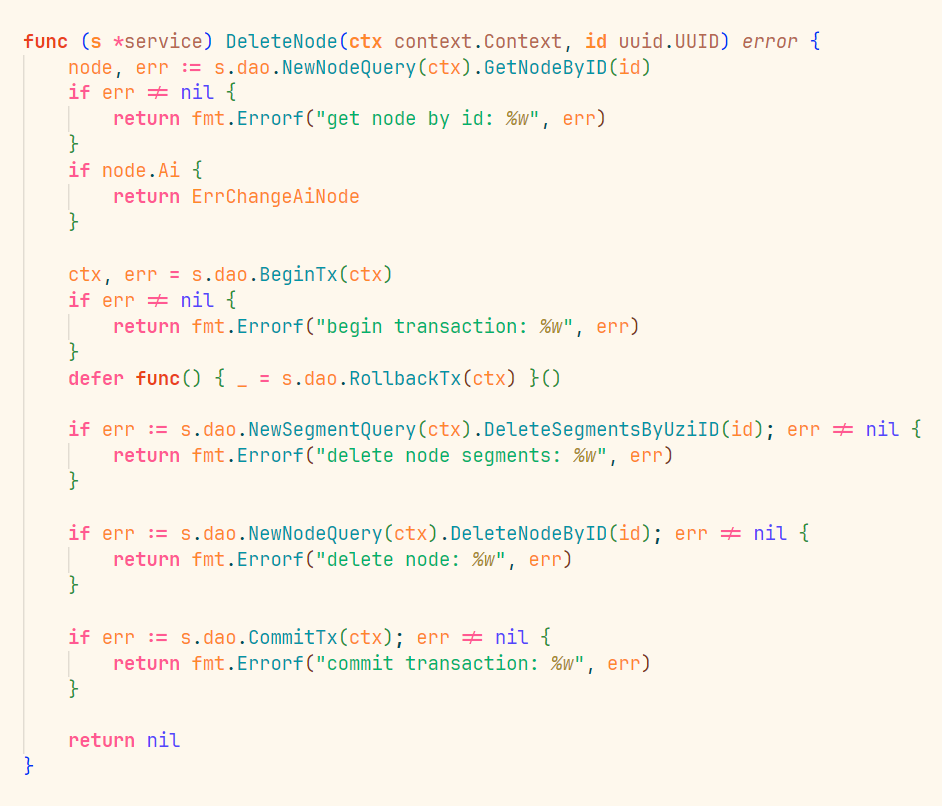
\includegraphics[width=.7\columnwidth]{./img/new/logical.png}%
	\end{center}
	\caption{Реализация удаления узла образования}%
	\label{pic:logical}%
\end{figure}

\subsection{Интерфейсы взаимодействия с внешними системами}
Для сохранения правила Dependency Inversion, все взаимодействия с внешними системами реализованы через интерфейсы, чей уровень
абстракции такого же уровня, что и уровень абстракции вызывающего интерфейс. Рассмотрим пример интерфейса для взаимодействия с 
базой данных.

\begin{figure}[H]%
	\begin{center}
		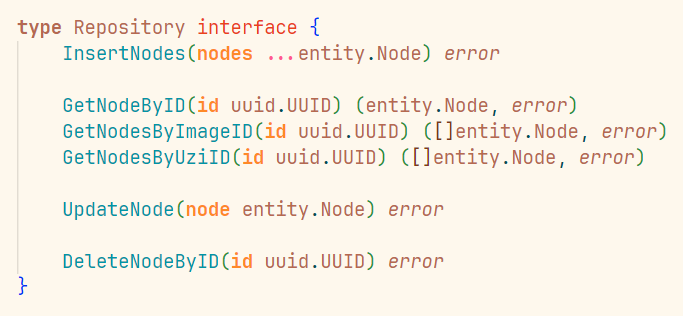
\includegraphics[width=.7\columnwidth]{./img/new/repository.png}%
	\end{center}
	\caption{Интерфейс взаимодействия с базой данных для узлов образований}%
	\label{pic:repository}%
\end{figure}

\subsection{Контракты микросервисов и API системы}
Все микросервисы взаимодействуют с друг другом посредством gRPC. Описания контрактов взаимодействия делается посредством
proto файлов. В них описываются rpc методы микросервиса, которые он реализует. Описаны ожидаемые структуры данных, которые 
используются в rpc методах.

\begin{figure}[H]%
	\begin{center}
		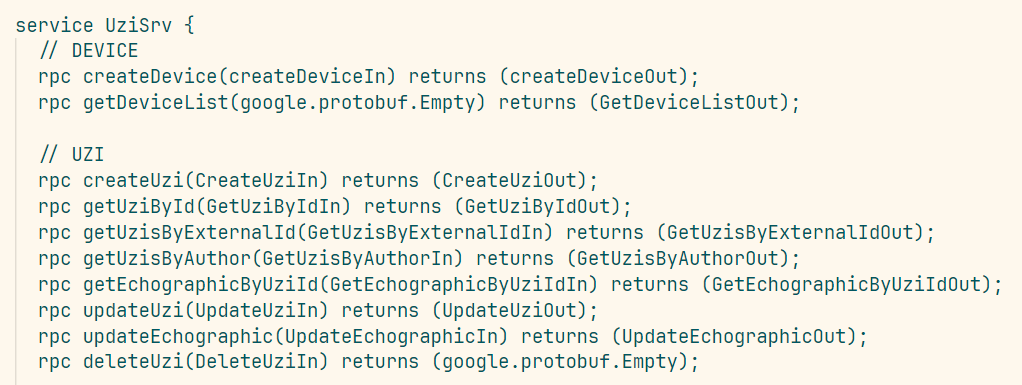
\includegraphics[width=.7\columnwidth]{./img/new/rpc_proto_1.png}%
	\end{center}
	\caption{Контракт взаимодействия с микросервисом управления УЗИ снимками}%
	\label{pic:rpc_proto_1}%
\end{figure}

\begin{figure}[H]%
	\begin{center}
		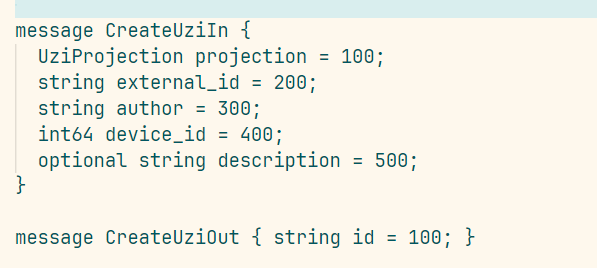
\includegraphics[width=.7\columnwidth]{./img/new/rpc_proto_2.png}%
	\end{center}
	\caption{Элементы контракта взаимодействия с микросервисом управления УЗИ снимками}%
	\label{pic:rpc_proto_2}%
\end{figure}

Далее рассмотрим API системы в целом. Этот API должен в полной мере покрывать все функциональные требования к системе, 
относящиеся к взаимодействию с системой. API системы описывается файлом в формате OpenAPI 3.0.

\begin{figure}[H]%
	\begin{center}
		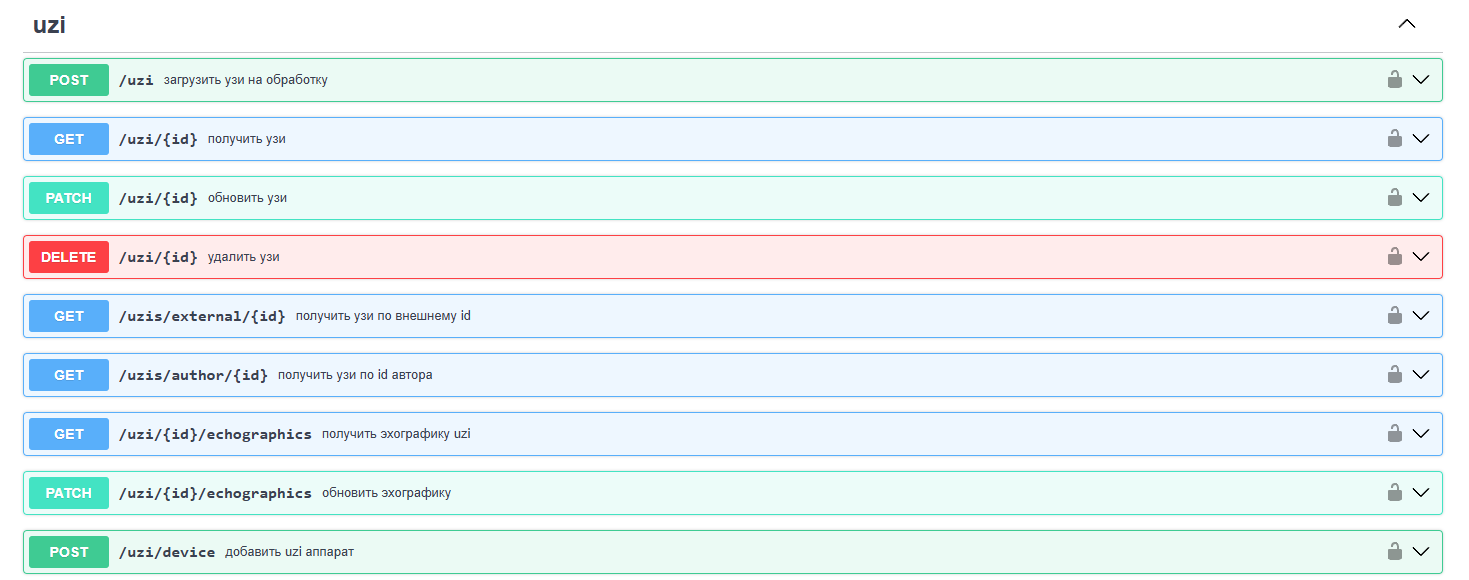
\includegraphics[width=.7\columnwidth]{./img/new/swagger_small.png}%
	\end{center}
	\caption{Часть API всей системы}%
	\label{pic:swagger_small}%
\end{figure}

\subsection{Топики стриминга сообщений для асинхронного общения}
Для использования асинхронного общения через RedPanda, создадим 3 топика:
\begin{itemize}
    \item \textbf{uziupload} - узи загруженно в S3. Запустит разбиение узи на кадры.
    \item \textbf{uzisplitted} - узи разбито на кадры. Запустит обработку узи нейро моделью. В топик пишет сервис управления УЗИ после разбиения узи на кадры.
    \item \textbf{uziprocessed} - узи обработанно нейромоделью. Узи сегментировано и классифицировано
\end{itemize}

\subsection{Структура хранилища узи снимков}
Структура S3 minio представлена в виде файловой системы, позволяет быстро искать необходимые файлы, зная их идентификатор. 
Микросервисы знают об устройстве S3, поэтому при необходимости передчи в другой микросервис узи снимков, достаточно передавать
id снимка.

\begin{figure}[H]%
	\begin{center}
		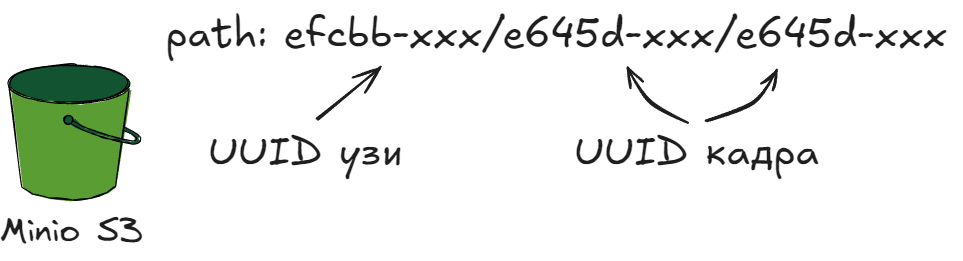
\includegraphics[width=.6\columnwidth]{./img/s3_arc.png}%
	\end{center}
	\caption{Структура S3 хранилища}%
	\label{pic:auth_model}%
\end{figure}


% В этой главе описывается, что и как было запрограммировано, отлажено, 
% протестировано, и что в результате получилось. Большинство работ должны 
% содержать приведенные ниже разделы. Но нужно учитывать, что точный состав 
% этой главы, как и других глав, зависит от специфики работы.

% Фрагменты программного кода в тексте необходимо выделять при помощи команды 
% \verb|\verb|. Многострочные листинги должны оформляться при помощи пакета 
% \verb|listings|. Пример:

% \begin{lstlisting}
% # let s x y z = x z (y z);;
% val s : ('a -> 'b -> 'c) -> ('a -> 'b) -> 'a -> 'c = <fun>
% # let k x y = x;;
% val k : 'a -> 'b -> 'a = <fun>
% # let i = s k k;;
% val i : '_a -> '_a = <fun>
% \end{lstlisting}

% Листинг \ref{lst:float-example} иллюстрирует использование выносных листингов.
% Листинг \ref{lst:HelloWorld.scala} показывает пример включения внешнего файла 
% в качестве листинга, в данном случае --- выносного.

% \begin{lstlisting}[
%   float=tb,frame=lines,label=lst:float-example,caption=Выносной листинг
% ]
% List myList = new List();
% Element myElement = new Element();
% myList.Append(myElement);
% \end{lstlisting}

% \lstinputlisting[
%   label=lst:HelloWorld.scala,
%   float=tb,frame=lines,
%   caption=Листинг из файла \texttt{HelloWorld.scala}
% ]{listings/HelloWorld.scala}


\section{Состав и структура реализованного программного обеспечения}

Реализованно серверное приложение, запускаемое как для локального использование, так и в 
серверном виде. Приложений отвечает на HTTP запросы, соответствует всем функциональным требованиям к системе.

\subsection{Структура приложения}
Приложение состоит из 5 микросервисов:
\begin{itemize}
  \item Composition API - точка входа в систему. Обрабатывает запросы от пользователя и передает их в соответствующие микросервисы.
  \item Микросервис Авторизации и Аутентификации - отвечает за аутентификацию и авторизацию пользователей.
  \item Микросервис Управления УЗИ снимками - отвечает за загрузку, разбиение на кадры, обработку узи нейромоделью.
  \item Микросервис Управления Медицинскими данными - отвечает за хранение и обработку медицинских данных.
  \item Микросервис Интеллектуальной части - отвечает за обработку узи нейромоделью.
\end{itemize}

Каждый микросервис написанный на golang содержит:
\begin{itemize}
  \item go.mod и go.sum файлы, описывающие библиотекчные зависимости для приложения
  \item sql файлы миграций. Сами миграции осуществлялись за счет утилиты Goose. SQL файлы в каждом микросервисе расположены по пути db/migrations
  \item proto файлы описывающие контракты для взаимодествия с внешними системами
  \item taskfile - файлы описывающие команды необходимые для локальной сборки микросервиса, миграции базы данных, генерации кода и т.д
  \item Dockerfile - файл для сборки docker образа микросервиса
  \item service.yml - файл содержащий конфигурацию сервиса
\end{itemize}


% Нужно охарактеризовать реализованное ПО: является ли оно настольной программной для Windows, 
% или веб-приложением в форме сайта/веб-сервиса, или модулем/подключаемой библиотекой, или 
% \dots. Также нужно перечислить, из чего оно состоит: какие исполняемые файлы и их назначение, 
% конфигурационные файлы, файлы баз данных, требования к программному и аппаратному окружению, и т.п.

% Если реализованное приложение достаточно обширно, этот раздел может быть
% разделен на несколько: один с общим описанием, и по одному на подсистемы самого
% верхнего уровня.

\section{Основные сценарии работы пользователя}
Основной сценарий работы ПО - отправка запросов на обработку узи изображений и полученние данных с
обработанных изображений. Для взаимодействием с сервисом предоставляется подробное swagger api.

\begin{figure}[H]%
	\begin{center}
		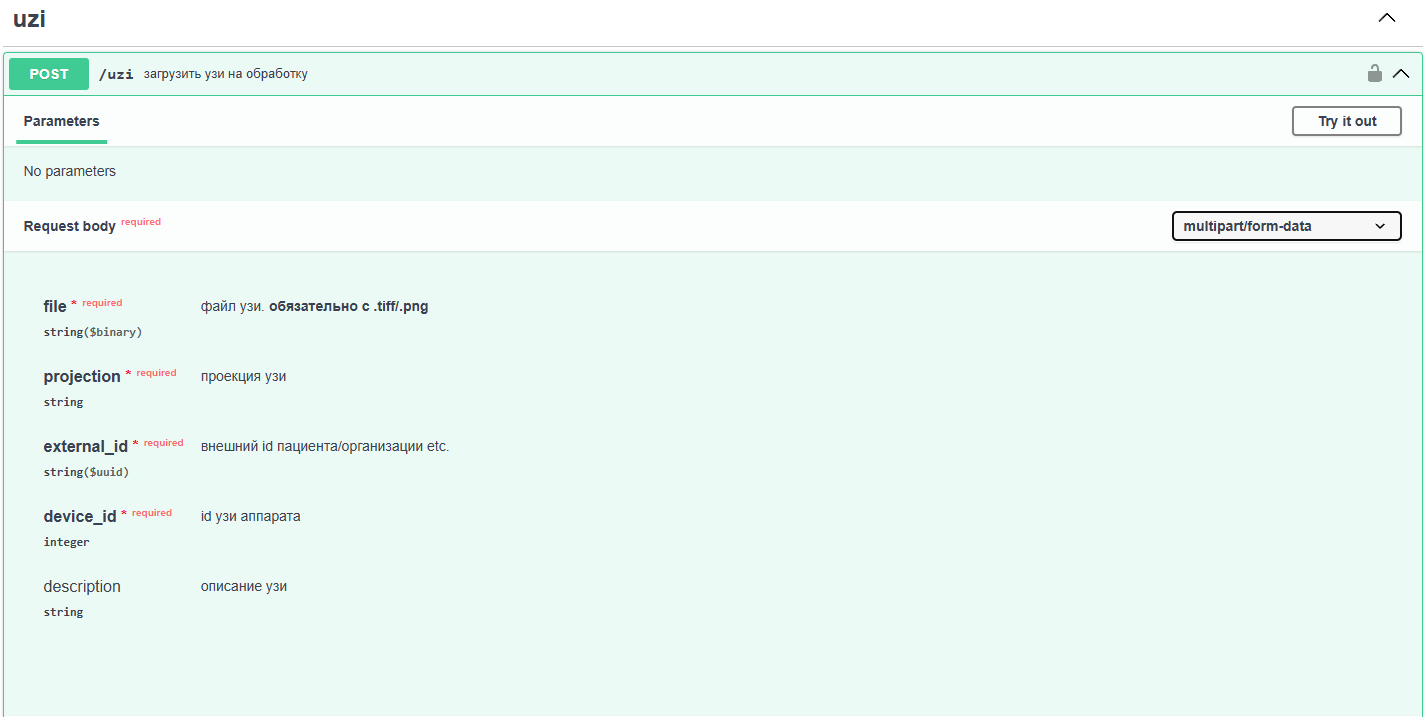
\includegraphics[width=.6\columnwidth]{./img/new/uzi_request.png}%
	\end{center}
	\caption{Запрос на загрузку и анализ uzi снимка}%
	\label{pic:uzi_request}%
\end{figure}

\begin{figure}[H]%
	\begin{center}
		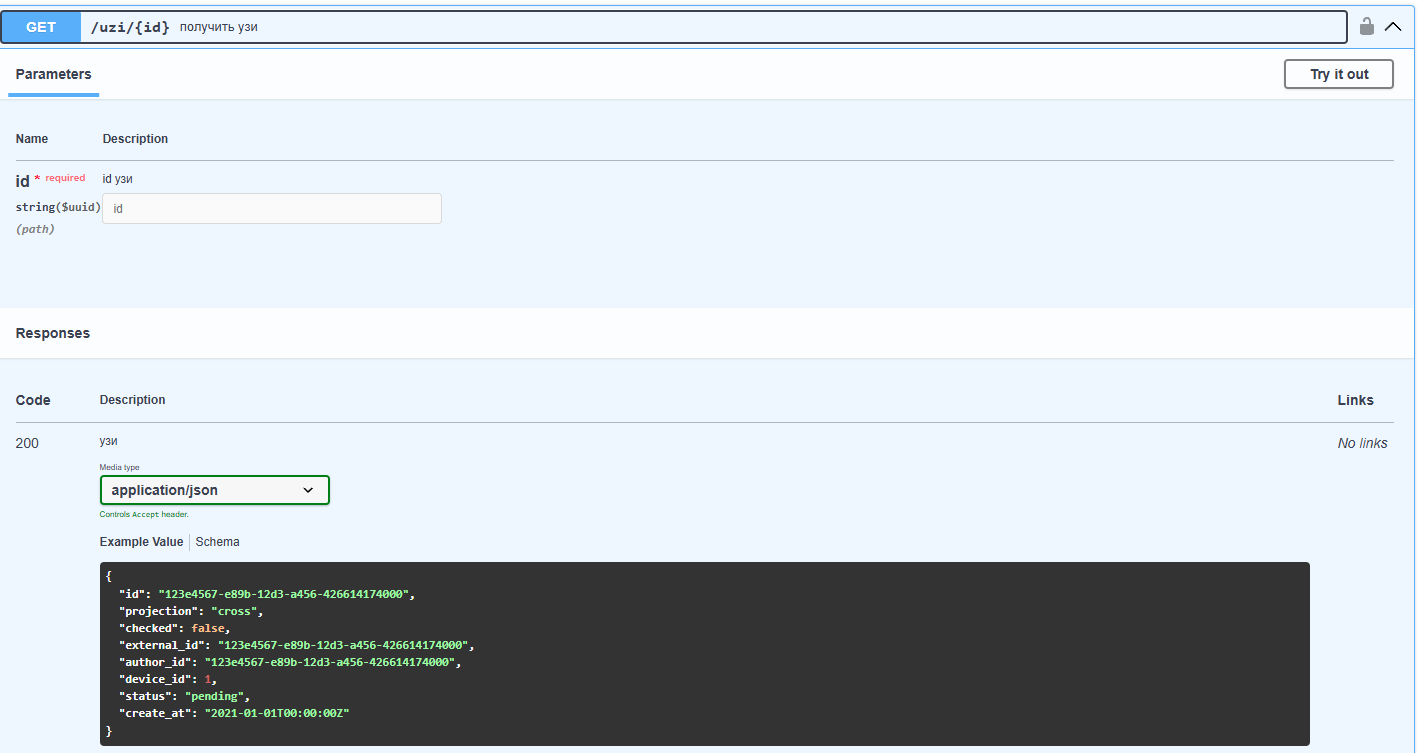
\includegraphics[width=.6\columnwidth]{./img/new/uzi_response.png}%
	\end{center}
	\caption{Запрос на получение информации по загруженному узи снимку}%
	\label{pic:uzi_response}%
\end{figure}

\section{Тестирование системы}
Тестирование программного обеспечения является критически важным этапом жизненного цикла разработки, 
обеспечивающим качество, надежность и соответствие требованиям готового продукта. Существует множество 
подходов к тестированию, каждый из которых решает определенные задачи и применяется на различных этапах 
разработки.

\subsection{Юнит тестирование}
Юнит тестирование представляет собой тестирование отдельных компонентов или модулей программы в изоляции 
от других частей системы. Этот вид тестирования обычно выполняется разработчиками и направлен на проверку 
корректности работы небольших участков кода, таких как функции, методы или классы.\\
Основные преимущества юнит тестирования включают раннее обнаружение дефектов, упрощение 
отладки и рефакторинга, а также создание документации к коду в виде тестовых сценариев. 
Для автоматизации модульного тестирования используются специальные фреймворки, 
такие как JUnit для Java, pytest для Python, или Jest для JavaScript.

Для модульного тестирования использовалась библиотека testing из стандартной библиотеки golang.
Пакет testing предоставляет необходимые инструменты для написания и выполнения тестов. 
Он интегрирован с утилитой go test, которая автоматически обнаруживает тесты в файлах с суффиксом \_test.go 
и выполняет их. Благодаря гибкой системе отчетов можно логировать дополнительную информацию, пропускать тесты при определенных условиях или запускать их параллельно для ускорения проверки.
С помощью флага -cover, можно выявить непротестированные участки.

Так же для проверки значений результатов использовалась библиотека testify. Она позволяет проверять значения результатов, такие как числа, строки, булевые значения, структуры данных и т.д.
Помимо проверки значений результатов, testify добавляет функционал мок объектов. Мок объекты - позволяют задать
поведения заранее определенного интерфейса. С помощью мок объекта, можно проверить что во время теста, у интерфейса
вызывается определенный метод с определенными параметрами. Помимо этого, мок объекту можно задать его поведение при
ответе, когда вызывается описанный метод.

Пример юнит тестирования в проекте:
\begin{figure}[H]%
	\begin{center}
		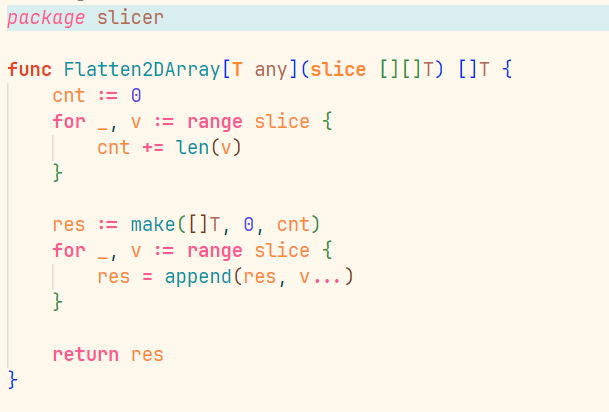
\includegraphics[width=.9\columnwidth]{./img/new/test_slice_1.png}%
	\end{center}
	\caption{Функция для для перевода 2-ух мерных массивов в 1-мерный}%
	\label{pic:test_slice_1}%
\end{figure}

Данная функция используется при разбиениее кинопетли на кадры. Библиотека для работы с tiff форматом, будет использовать
двумерный массив, который нам нужно будет перевести в 1-мерный.

Тесты для данной функции:
\begin{figure}[H]%
	\begin{center}
		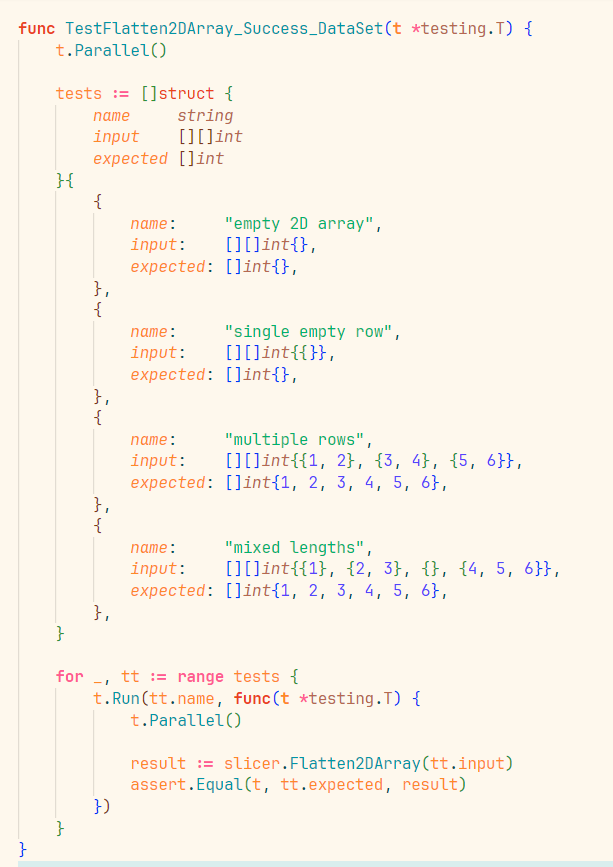
\includegraphics[width=.9\columnwidth]{./img/new/test_slice_2.png}%
	\end{center}
	\caption{Юнит тесты на функцию Flatten2DArray}%
	\label{pic:test_slice_2}%
\end{figure}

Данный тест используется методику "Табличных тестов". Испольуется массив анонимных структур, в которых описываются ряд сценариев
для тестирования.

\subsection{Интеграционное тестирование}
Интеграционное тестирование представляет собой тестирование взаимодействия между различными компонентами или модулями программы. 
Этот вид тестирования обычно выполняется разработчиками и направлен на проверку корректности взаимодействия между различными частями системы.\\

Основные преимущества интеграционного тестирования включают раннее обнаружение дефектов, упрощение отладки и рефакторинга, а также создание 
документации к коду в виде тестовых сценариев.

Основным сценарием интеграционного тестирования, является тестирования взаимодействия микросервиса с базой данных или брокером сообщений.\\
Взаимодействие с базой данных происходит в слое Репозитория. От основной логики приложения он отделен интерфейсом. 

\begin{figure}[H]%
	\begin{center}
		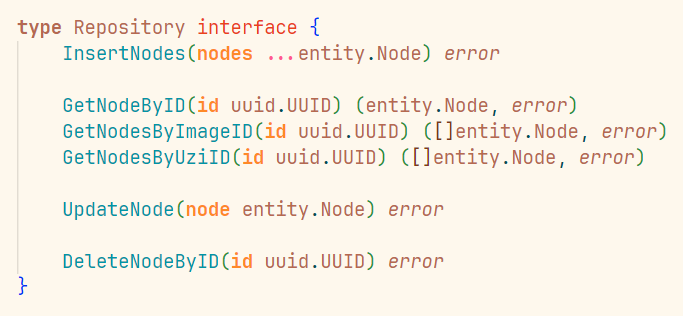
\includegraphics[width=.7\columnwidth]{./img/new/repository.png}%
	\end{center}
	\caption{Интерфейс взаимодействия с базой данных для узлов образований}%
	\label{pic:repository}%
\end{figure}

Реализация интерфейса непосредственно взаимодействует с базой данных:
\begin{figure}[H]%
	\begin{center}
		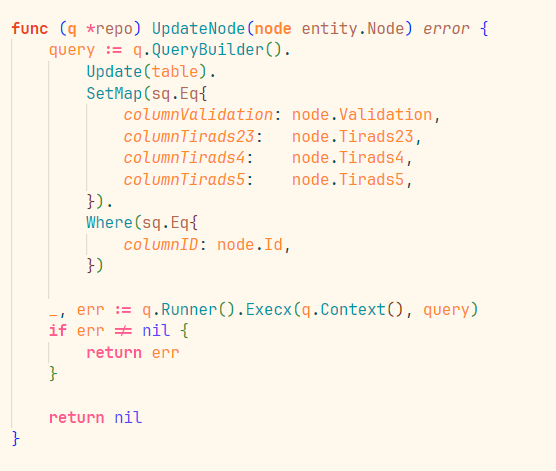
\includegraphics[width=.7\columnwidth]{./img/new/repostitory_update.png}%
	\end{center}
	\caption{Интерфейс взаимодействия с базой данных для обновления узла образований}%
	\label{pic:repository_update}%
\end{figure}

Тесты на слой взаимодействия с базой данных, прямым образом проверяют корректность работы сервиса с базой данных,
так как более нигде кроме слоя репозитория, сервис с базой данных не взаимодействует.
\begin{figure}[H]%
	\begin{center}
		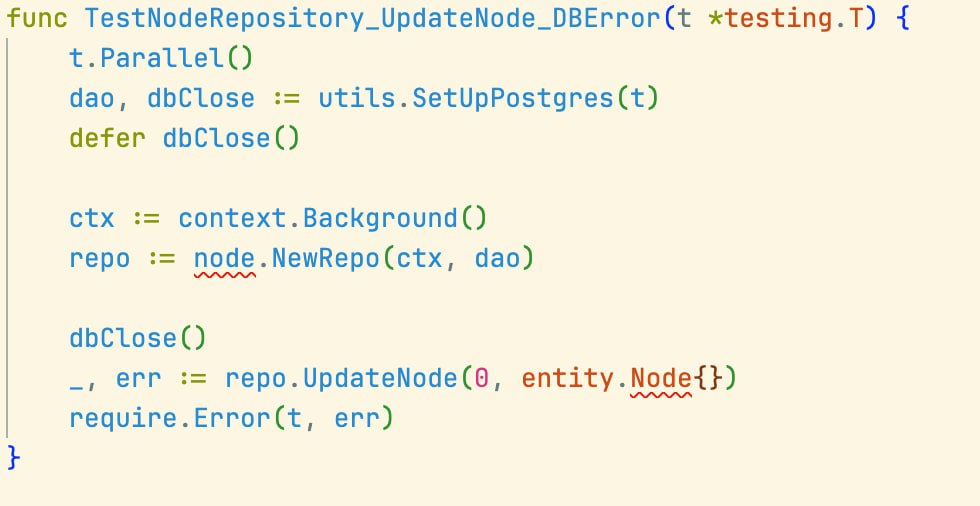
\includegraphics[width=.7\columnwidth]{./img/new/integration_test.png}%
	\end{center}
	\caption{Тесты проверяющий отказ базы данных при запросе}%
	\label{pic:repository_test}%
\end{figure}

\section{Сквозное тестирование}
Сквозное тестирование представляет собой тестирование взаимодействия между различными компонентами или модулями программы. 
Этот вид тестирования обычно выполняется разработчиками и направлен на проверку корректности взаимодействия между различными частями системы.\\

Основные преимущества сквозного тестирования включают раннее обнаружение дефектов, упрощение отладки и рефакторинга, а также создание 
документации к коду в виде тестовых сценариев.

Так как каждый микросервис предоставляет свой контракт взаимодействия, то для хорошего покрытия сквозного тестирования, требуется тест на каждую ручку.
Рассмотрим пример сквозного тестирования на примере микросервиса управления УЗИ снимками. Микросервис предоставляет контракт,
позволяющий ставить узи на обработку, а затем получаеть результаты обработки в различных разрезах.\\
Обработку узи снимка можно представить в следующем виде:
\begin{figure}[H]%
	\begin{center}
		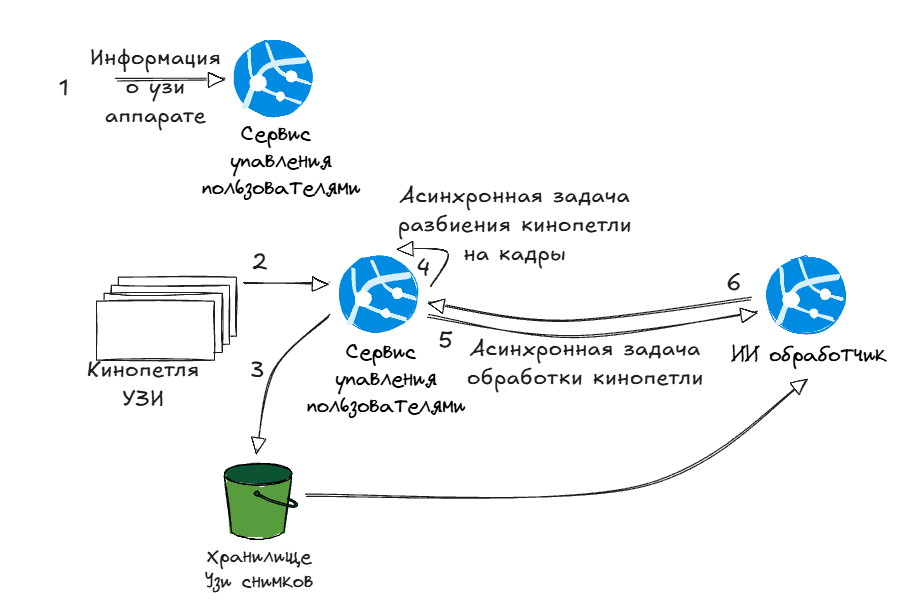
\includegraphics[width=.7\columnwidth]{./img/new/uzi_flow.png}%
	\end{center}
	\caption{Схема обработки узи снимка}%
	\label{pic:uzi_flow}%
\end{figure}

Разобьем на следующие этапы:
\begin{itemize}
  \item Загрузка информации о узи аппарате
  \item Загрузка узи снимка в S3
  \item Разбиение узи снимка на кадры
  \item Обработка узи снимка нейромоделью
  \item Получение результатов обработки узи снимка
\end{itemize}

Каждая группа ручек из контракта проверяет определенный набор этапов. Мы не можем проводить тесты на системе с уже обработанным снимком,
так как это не будет отражать реальное поведение системы в использовании. Поэтому для каждого теста, нужно выполнения соответствующих ряда этапов.
Для примера возьмем ручки, проверяющие разбиение узи снимка на кадры. Для этих тестов обработка нейромоделью узи не требуется, так как проверяться не будет,
но оно увеличит время проведения тестов.

Для решения данной задачи применем паттерн "Цепочка ответственности". В нем каждый этап выделяется в отдельную состовляющую, имеющую зависимости от остальных этапов,
если такие присутствуют. Использование данного подхода, позволит индивидуально или группе тестов указывать необходимые для них этапы, автоматизированно выполнять их, 
собирая информацию о поведении системы, и не выполнять лишние этапы, нагружая систему лишним трафиком.
\begin{figure}[H]%
	\begin{center}
		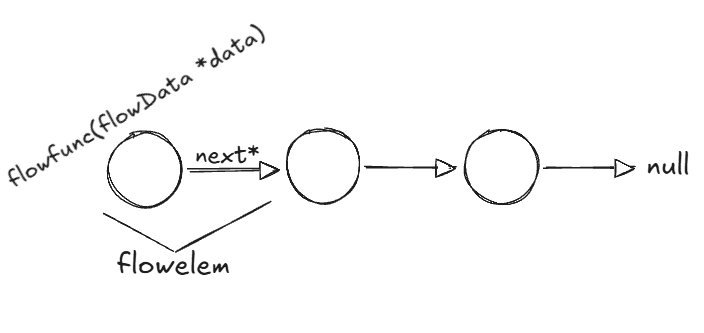
\includegraphics[width=.7\columnwidth]{./img/new/flow_test.png}%
	\end{center}
	\caption{Цепочка ответственности для сквозного тестирования}%
	\label{pic:flow_test}%
\end{figure}

Пример сквозного тестирования для разбиения узи снимка на кадры:
\begin{figure}[H]%
	\begin{center}
		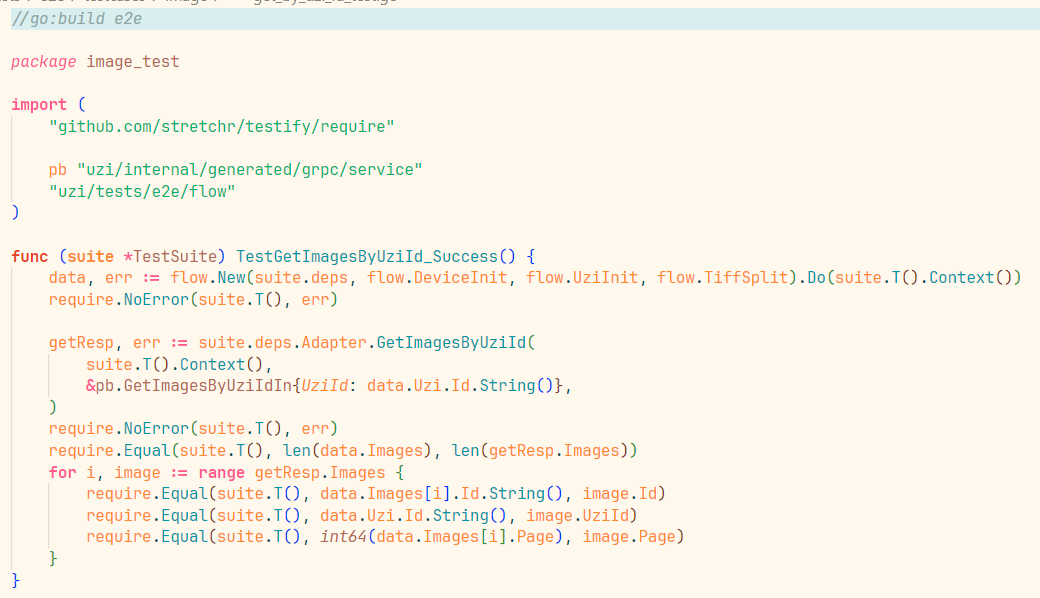
\includegraphics[width=.7\columnwidth]{./img/new/e2e_test.png}%
	\end{center}
	\caption{Сквозное тестирование для разбиения узи снимка на кадры}%
	\label{pic:e2e_test}%
\end{figure}
% Нужно помнить, что пользователем может быть не только <<менеджер>> или <<человек в белом халате>>, 
% но и другой программист. Последнее относится, в первую очередь, к реализованным библиотекам. 
% Для <<обычных>> приложений нередко бывают пользователи нескольких категорий --- например, обычный 
% пользователь и администратор. Для каждой категории нужно описать, как выполняются основные функции, 
% предпочтительно, с помощью серии скрин-шотов. Однако считается плохим тоном вставлять длинную вереницу 
% из скрин-шотов: если их много, большую часть нужно выносить в приложение. Для \textit{этого} раздела 
% нормальной является плотность скрин-шотов из расчета: 1 страница скрин-шотов на 1-2 страницы текста.


\section{Выводы}
В результате проведенного анализа, моделирования и проектирования реализованна система "Интеллектуальный ассистент врача". 
Примененные для реализации интсрументы и технологии соответствуют выбранным в прошлой главе.


Серверное приложение состоит из 4 микросервисов связанных с друг другом посредством синхронного и асинхронного общения. Примененный паттерн Composition-Api 
обеспечивает единую точку входа для взаимодействия с системой. Для использования системы представлено понятное API.


В рамках тестирования, написаны модульные, интеграционные и сквозные тесты. Для полноценного свозного тестирования системы, освновные сценарии использования
разбиты на обособленные шаги, реализован механизм воспроизведения определенных шагов для каждого теста в отдельности. 

% Следует перечислить, какие практические результаты были получены, а именно: какое 
% программное или иное обеспечение было создано. В число результатов могут входить, 
% например, методики тестирования, тестовые примеры (для проверки корректности/оценки 
% характеристик тех или иных алгоритмов) и др. По каждому результату следует сделать вывод, 
% насколько он отличается от известных промышленных аналогов и исследовательских прототипов.



%%% Local Variables:
%%% TeX-engine: xetex
%%% eval: (setq-local TeX-master (concat "../" (seq-find (-cut string-match ".*-3-pz\.tex$" <>) (directory-files ".."))))
%%% End:
